%-------------------------------------------------------------------------------
%                                PREAMBLE
%-------------------------------------------------------------------------------
\documentclass[usenames,dvipsnames,svgnames,10pt,aspectratio=169]{beamer}
%
\usefonttheme{professionalfonts}
% This theme uses TIKZ: compile twice with PDFLaTeX or LuaLaTeX.
%
%  Options:
%  - [clean]:    clean slides, i.e. logos and footbar are removed
%  - [kth]:      footbar style inspierd to the official KTH template
%  - [nicewave]: a different style of wave is used (not approved by FLOW)
%
\usetheme[clean]{flow}

\usepackage{tikz}
\usetikzlibrary{arrows}
\usetikzlibrary{shapes.geometric, math, positioning, calc, patterns, angles, quotes}
\newcommand{\semaphore}[3]{% #1: color of circle, 
                           % #2: color of semicircle
                           % #3: angle of semicircle 
  \tikz[node distance=0mm,baseline]
       {
         \node (s1) [circle, fill=#1, minimum size=6mm] {};
         \node      [semicircle, fill=#2, 
           inner sep=0pt, outer sep=0pt, minimum size=3mm,
           anchor=south,
           at={(s1.center)}, rotate=#3] {};
       }
}

\usepackage[]{circuitikz}

\usepackage{pgfplots}
\usepgfplotslibrary{polar}

\usepackage{hyperref,graphicx,lmodern}
\usepackage[utf8]{inputenc}
\usepackage{media9}
\usepackage{xcolor}
\usepackage{stmaryrd}
\usepackage{nicefrac}
\usepackage{multimedia}
\usepackage{multicol}
\usepackage{upgreek}
\usepackage[]{bm}
\usepackage[]{url}
\usepackage[]{animate}
\usepackage{amsmath}

\graphicspath{{imgs/}}
\setbeamertemplate{blocks}[rounded][shadow=true]


%-------------------------------------------------------------------------------
%                                TITLE PAGE
%-------------------------------------------------------------------------------
\title[Nonlinear physics] % Short title used in footline
{
	Elementary bifurcations
}

\author[J.-Ch.~Loiseau] % Presenting author in short form used in footline
{
	\underline{Jean-Christophe Loiseau}
}
% - Give the names in the same order as the appear in the paper.
% - Underline the presenting author.

\institute[unused]
{
	\url{jean-christophe.loiseau@ensam.eu} \\
	Laboratoire DynFluid \\
	Arts et M\'etiers, France.
}
% Keep it simple, no one is interested in your street address.

% University logo(s)
\logot{\includegraphics[width=.128\paperwidth]{DynFluid_logo}}  % Top logo
\logob{\includegraphics[width=0.128\paperwidth]{ENSAM_logo}} % Bottom logo
% \logoc[{\includegraphics[width=.128\paperwidth]{limsi}}]{\includegraphics[width=.128\paperwidth]{limsi}} % Corner logo
%
% Cover image: \cvrimg{x position}{y position}{cover image}
\cvrimg{.77}{.8}{\includegraphics[width=.4\paperwidth]{cover.png}}

\date[unused]{Physique non-lin\'eaire -- 2019-2020}

\begin{document}

\titleframe	% Print the title as the first slide

%-------------------------------------------------------------------------------
%                           PRESENTATION SLIDES
%-------------------------------------------------------------------------------

\begin{frame}[t, c]{First-order systems}{Flow on the real number line}
  \begin{minipage}{.48\textwidth}
    \begin{block}{\centering \textbf{First-order systems}}

    \[ \dot{x} = f(x) \]
    \end{block}

    \medskip

    \begin{itemize}
    \item $x(t)$ a real-valued function of time $t$,

      \medskip

    \item $f(x) : \mathbb{R} \to \mathbb{R}$ a smooth real-valued function of $x$ and does not explicitely depend on time $t$.
    \end{itemize}
  \end{minipage}%
  \hfill
  \begin{minipage}{.48\textwidth}
    \[
    \begin{aligned}
      \dot{x} & = \sum_{k=0}^N a_k x^k, \quad \text{with } a_k \in \mathbb{R} \quad \forall k \\
      \dot{x} & = \sin x \\
      \dot{x} & = \dfrac{1}{x} \\
      \vdots
    \end{aligned}
    \]
  \end{minipage}

  \vspace{1cm}
\end{frame}

\begin{frame}[t, c]{Parameterized first-order systems}{Elementary bifurcations}
  \begin{minipage}{.48\textwidth}
    \begin{block}{\centering \textbf{Parameterized first-order systems}}

    \[ \dot{x} = f(x, \mu) \]
    \end{block}

    \medskip

    \begin{itemize}
    \item $x(t)$ a real-valued function of time $t$,

      \medskip

    \item $\mu$ a real-valued parameter (or vector of parameters),

      \medskip

    \item $f(x, \mu) : \mathbb{R} \times \mathbb{R} \to \mathbb{R}$ a smooth real-valued function of $x$ and $\mu$ which does not explicitely depend on time $t$.
    \end{itemize}
  \end{minipage}%
  \hfill
  \begin{minipage}{.48\textwidth}
    \[
    \begin{aligned}
      \dot{x} & = \mu - x^2 \\
      \dot{x} & = \mu x - x^2 \\
      \dot{x} & = \mu x + x^3 \\
      \dot{x} & = \mu - \sin(x) \\
      \vdots
    \end{aligned}
    \]
  \end{minipage}

  \vspace{1cm}
\end{frame}

\begin{frame}[t, c]{Parameterized first-order systems}{Motivating example : Rudimentary model of solid-state lasers}
  \begin{minipage}{.58\textwidth}
    \begin{block}{\centering \textbf{Haken's model} (1983)}
      \[
      \begin{aligned}
        \dot{n} & = \text{gain} - \text{loss} \\
        & = GnN(t) - kn
      \end{aligned}
      \]
    \end{block}

    \bigskip

    In the model above, we have :
    \begin{itemize}
    \item $n(t)$ is the number of photons,
    \item $N(t)$ is the number of excited atoms,
    \item $G$ is the gain coefficient,
    \item $k$ is the rate at which photons escape.
    \end{itemize}
  \end{minipage}%
  \hfill
  \begin{minipage}{.38\textwidth}
    \centering
    \includegraphics[width=\textwidth]{laser}
  \end{minipage}

  \vspace{1cm}
\end{frame}

\begin{frame}[t, c]{Parameterized first-order systems}{Motivating example : Rudimentary model of solid-state lasers}
  \begin{minipage}{.58\textwidth}
    \begin{overprint}
      \onslide<1>
      Assuming that $N(t) = N_0 - \alpha n$ (with $\alpha > 0$), the model becomes
      %
      \[
      \begin{aligned}
        \dot{n} & = Gn(N_0 - \alpha n) - kn \\
        & = (GN_0 - k) n - (\alpha G) n^2.
      \end{aligned}
      \]
      
      \medskip
      
      The number of photons $n(t)$ in the laser thus appears to depend on four parameters $G$, $N_0$, $k$ and $\alpha$.

      \onslide<2>
      Rescaling time as $t \to \tau t$ and choose the time scale $\tau$ appropriately, the equation becomes
      %
      \[
      \begin{aligned}
        \dot{n} & = \dfrac{G N_0 - k}{\alpha G} n - n^2 \\
        & = \mu n - n^2.
      \end{aligned}
      \]

      The dynamics of the system effectively depend on a single parameter $\mu$.
    \end{overprint}
  \end{minipage}%
  \hfill
  \begin{minipage}{.38\textwidth}
    \begin{overprint}
      \onslide<2>
      \centering
      \textbf{Solution}

      \[n(t) = \dfrac{\mu n_0}{(\mu - n_0) e^{-\mu t} + n_0} \]
    \end{overprint}
  \end{minipage}

  %\vspace{1cm}
\end{frame}

\begin{frame}[t, c]{Parameterized first-order systems}{Motivating example : Rudimentary model of solid-state lasers}
  \begin{minipage}{.32\textwidth}
    \centering
    \begin{tikzpicture}[domain=0:2]
      \draw[->] (-0.25, 0) -- (2, 0) node[below] {$n$};
      \draw[->] (0, -2) -- (0, 2) node[left] {$\dot{n}$};

      \draw[gray, line width=0.5mm, domain=0:1.18614] plot (\x, {-0.5*\x - \x^2});

      \node[circle,fill=black,inner sep=0pt,minimum size=4pt] (a) at (0, 0) {};
      \node[rotate=90, inner sep=0pt] () at (0.25, 0) {\tikz\draw[-triangle 45](0, 0) ;};

    \end{tikzpicture}

    $$\mu = -\dfrac{1}{2}$$
  \end{minipage}%
  \hfill
  \begin{minipage}{.32\textwidth}
    \centering
    \begin{tikzpicture}[domain=0:2]
      \draw[->] (-0.25, 0) -- (2, 0) node[below] {$n$};
      \draw[->] (0, -2) -- (0, 2) node[left] {$\dot{n}$};

      \draw[gray, line width=0.5mm, domain=0:1.414] plot (\x, {- \x^2});

      \node[circle,fill=black,inner sep=0pt,minimum size=4pt] (a) at (0, 0) {};
      \node[rotate=90, inner sep=0pt] () at (0.25, 0) {\tikz\draw[-triangle 45](0, 0) ;};

    \end{tikzpicture}

    $$\mu = 0$$
  \end{minipage}%
  \hfill
  \begin{minipage}{.32\textwidth}
    \centering
    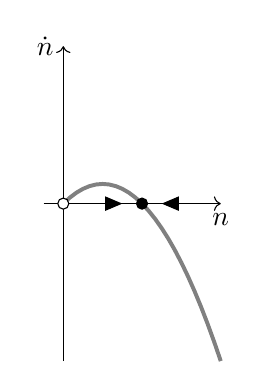
\begin{tikzpicture}[domain=0:2]
      \draw[->] (-0.25, 0) -- (2, 0) node[below] {$n$};
      \draw[->] (0, -2) -- (0, 2) node[left] {$\dot{n}$};

      \draw[gray, line width=0.5mm, domain=0:2] plot (\x, {\x - \x^2});

      \node[circle,fill=white, draw=black, inner sep=0pt,minimum size=4pt] (a) at (0, 0) {};
      \node[rotate=-90, inner sep=0pt] () at (0.75, 0) {\tikz\draw[-triangle 45](0, 0) ;};

      \node[circle, fill=black, draw=black, inner sep=0pt,minimum size=4pt] (a) at (1, 0) {};
      \node[rotate=90, inner sep=0pt] () at (1.25, 0) {\tikz\draw[-triangle 45](0, 0) ;};

    \end{tikzpicture}

    $$\mu = 1$$
  \end{minipage}

  \vspace{1cm}
\end{frame}

\begin{frame}[t, c]{Parameterized first-order systems}{Motivating example : Rudimentary model of solid-state lasers}
  \begin{minipage}{.68\textwidth}
    \begin{overprint}
      \only<1->
      For $\mu < 0$, $n = 0$ is a stable fixed point.
      No stimulated emission happens and the laser acts as a lamp.

      \bigskip

      \onslide<2>
      For $\mu > 0$, $n = 0$ is no longer stable. 
      The process of stimulated emission sets in and the laser behave as expected.

      \bigskip

      \begin{block}{}
        This drastic change of dynamics as the parameter $\mu$ exceeds a critical threshold is known as a \textbf{\alert{bifurcation}}.
      \end{block}

    \end{overprint}
  \end{minipage}%
  \hfill
  \begin{minipage}{.28\textwidth}
    \begin{overprint}
      \onslide<1>
      \centering
      \begin{tikzpicture}[domain=0:2]
        \draw[->] (-0.25, 0) -- (2, 0) node[below] {$n$};
        \draw[->] (0, -2) -- (0, 2) node[left] {$\dot{n}$};
        
        \draw[gray, line width=0.5mm, domain=0:1.18614] plot (\x, {-0.5*\x - \x^2});
        
        \node[circle,fill=black,inner sep=0pt,minimum size=4pt] (a) at (0, 0) {};
        \node[rotate=90, inner sep=0pt] () at (0.25, 0) {\tikz\draw[-triangle 45](0, 0) ;};
        
      \end{tikzpicture}

      $$\mu < 0$$

      \onslide<2>
      \centering
      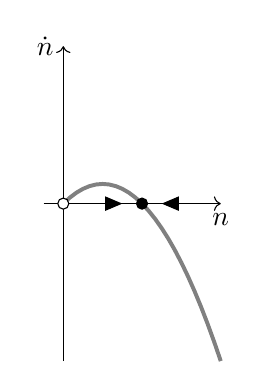
\begin{tikzpicture}[domain=0:2]
        \draw[->] (-0.25, 0) -- (2, 0) node[below] {$n$};
        \draw[->] (0, -2) -- (0, 2) node[left] {$\dot{n}$};
        
        \draw[gray, line width=0.5mm, domain=0:2] plot (\x, {\x - \x^2});
        
        \node[circle,fill=white, draw=black, inner sep=0pt,minimum size=4pt] (a) at (0, 0) {};
        \node[rotate=-90, inner sep=0pt] () at (0.75, 0) {\tikz\draw[-triangle 45](0, 0) ;};
        
        \node[circle, fill=black, draw=black, inner sep=0pt,minimum size=4pt] (a) at (1, 0) {};
        \node[rotate=90, inner sep=0pt] () at (1.25, 0) {\tikz\draw[-triangle 45](0, 0) ;};
        
      \end{tikzpicture}
      
      $$\mu > 0$$
      
    \end{overprint}
  \end{minipage}

  \vspace{1cm}
\end{frame}

\begin{frame}[t, c]{Transcritical bifurcation}{The law of equivalent exchange}
  \begin{minipage}{.32\textwidth}
    \centering
    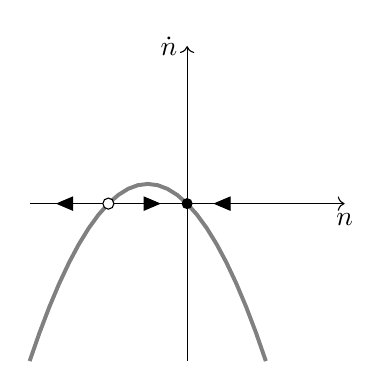
\begin{tikzpicture}[domain=-2:2]
      \draw[->] (-2, 0) -- (2, 0) node[below] {$n$};
      \draw[->] (0, -2) -- (0, 2) node[left] {$\dot{n}$};

      \draw[gray, line width=0.5mm, domain=-2:1] plot (\x, {-\x - \x*\x});

      \node[circle,fill=black,inner sep=0pt,minimum size=4pt] (a) at (0, 0) {};
      \node[rotate=90, inner sep=0pt] () at (0.3333, 0) {\tikz\draw[-triangle 45](0, 0) ;};

      \node[circle,fill=white, draw=black, inner sep=0pt,minimum size=4pt] (a) at (-1, 0) {};
      \node[rotate=-90, inner sep=0pt] () at (-0.3333, 0) {\tikz\draw[-triangle 45](0, 0) ;};
      \node[rotate=90, inner sep=0pt] () at (-1.6666, 0) {\tikz\draw[-triangle 45](0, 0) ;};

    \end{tikzpicture}

    $$\mu = -1$$
  \end{minipage}%
  \hfill
  \begin{minipage}{.32\textwidth}
    \centering
    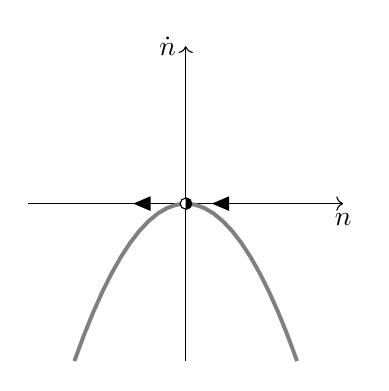
\begin{tikzpicture}[domain=-2:2]
      \draw[->] (-2, 0) -- (2, 0) node[below] {$n$};
      \draw[->] (0, -2) -- (0, 2) node[left] {$\dot{n}$};

      \draw[gray, line width=0.5mm, domain=-1.414:1.414] plot (\x, {-\x*\x});

      \node[circle, fill=white, draw=black, inner sep=0pt, minimum size=4pt] (a) at (0, 0) {};
      \node[semicircle, fill=black, draw=black, inner sep=0pt, minimum size=2pt, rotate=-90, anchor=south] (a) at (0, 0) {};
      \node[rotate=90, inner sep=0pt] () at (0.333, 0) {\tikz\draw[-triangle 45](0, 0) ;};
      \node[rotate=90, inner sep=0pt] () at (-0.666, 0) {\tikz\draw[-triangle 45](0, 0) ;};

    \end{tikzpicture}

    $$\mu = 0$$
  \end{minipage}%
  \hfill
  \begin{minipage}{.32\textwidth}
    \centering
    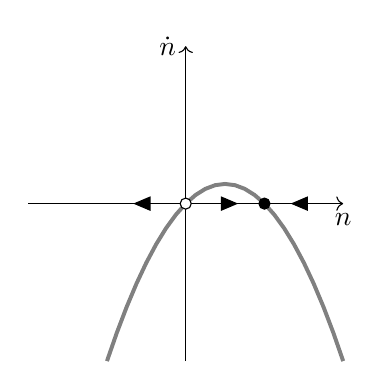
\begin{tikzpicture}[domain=-2:2]
      \draw[->] (-2, 0) -- (2, 0) node[below] {$n$};
      \draw[->] (0, -2) -- (0, 2) node[left] {$\dot{n}$};

      \draw[gray, line width=0.5mm, domain=-1:2] plot (\x, {\x - \x*\x});

      \node[circle,fill=white, draw=black, inner sep=0pt,minimum size=4pt] (a) at (0, 0) {};
      \node[rotate=-90, inner sep=0pt] () at (0.666, 0) {\tikz\draw[-triangle 45](0, 0) ;};
      \node[rotate=90, inner sep=0pt] () at (-0.666, 0) {\tikz\draw[-triangle 45](0, 0) ;};

      \node[circle, fill=black, draw=black, inner sep=0pt,minimum size=4pt] (a) at (1, 0) {};
      \node[rotate=90, inner sep=0pt] () at (1.333, 0) {\tikz\draw[-triangle 45](0, 0) ;};

    \end{tikzpicture}

    $$\mu = 1$$
  \end{minipage}

  \vspace{1cm}
\end{frame}


\begin{frame}[t, c]{Transcritical bifurcation}{The law of equivalent exchange}
  \begin{minipage}{.48\textwidth}
    \begin{block}{\centering \alert{\textbf{Transcritical bifurcation}}}
      \centering
      \medskip

      \( \dot{x} = \mu x - x^2 \)
    \end{block}

    \bigskip

    \begin{itemize}
    \item Two fixed points given by $x_1 = 0$ and $x_2 = \mu$ exist for all $\mu$.

      \medskip

    \item At $\mu = 0$ they collide and exchange their stability properties for $\mu > 0$.
    \end{itemize}

  \end{minipage}%
  \hfill
  \begin{minipage}{.48\textwidth}
    \centering
    \begin{tikzpicture}
      \draw[->] (-3, 0) -- (3, 0) node[below] {$\mu$};
      \draw[->] (0, -1.5) -- (0, 1.5) node[left] {$x^*$};

      \draw[blue, line width=0.5mm, domain=-2:0] plot (\x, {0*\x});
      \draw[blue, dashed, line width=0.5mm, domain=0:2] plot (\x, {0*\x});

      \draw[blue, dashed, line width=0.5mm, domain=-2:0] plot (\x, {0.6666*\x});
      \draw[blue, line width=0.5mm, domain=0:2] plot (\x, {0.6666*\x});

    \end{tikzpicture}
  \end{minipage}

  \vspace{1cm}
\end{frame}

\begin{frame}[t, c]{Saddle-node bifurcation}{Fixed points appearing ''out of the clear blue sky''}
  \begin{minipage}{.48\textwidth}
    \begin{block}{\centering \alert{\textbf{Saddle-node bifurcation}}}
      \centering

      \medskip

      \( \dot{x} = \mu - x^2 \)
    \end{block}

    \bigskip

    \begin{itemize}
    \item For $\mu < 0$, no fixed points exist.

      \medskip

    \item As $\mu$ becomes positive, two fixed points given by $x_{1, 2} = \pm \sqrt{\mu}$ appear out of thin air.

      \medskip

    \item One of these fixed points is linearly stable while the other is linearly unstable.
    \end{itemize}
  \end{minipage}%
  \hfill
  \begin{minipage}{.48\textwidth}
    \centering
    \begin{tikzpicture}
      \draw[->] (-3, 0) -- (3, 0) node[below] {$\mu$};
      \draw[->] (0, -1.5) -- (0, 1.5) node[left] {$x^*$};

      \draw[blue, line width=0.5mm, domain=0:2, samples=401] plot (\x, {0.6666*\x^(1/2)});
      \draw[blue, dashed, line width=0.5mm, domain=0:2, samples=401] plot (\x, -{0.6666*\x^(1/2)});

    \end{tikzpicture}
  \end{minipage}

  \vspace{1cm}
\end{frame}

\begin{frame}[t, c]{Saddle-node bifurcation}{Fixed points appearing ''out of the clear blue sky''}
  \begin{minipage}{.32\textwidth}
    \centering
    \begin{tikzpicture}[domain=-2:2]
      \draw[->] (-2, 0) -- (2, 0) node[below] {$x$};
      \draw[->] (0, -2) -- (0, 2) node[left] {$\dot{x}$};

      \draw[gray, line width=0.5mm, domain=-1:1] plot (\x, {-1 - \x*\x});

      \node[rotate=90, inner sep=0pt] () at (-0.666, 0) {\tikz\draw[-triangle 45](0, 0) ;};

      \node[rotate=90, inner sep=0pt] () at (0.5, 0) {\tikz\draw[-triangle 45](0, 0) ;};

    \end{tikzpicture}

    $$\mu = -1$$

  \end{minipage}%
  \hfill
  \begin{minipage}{.32\textwidth}
    \centering
    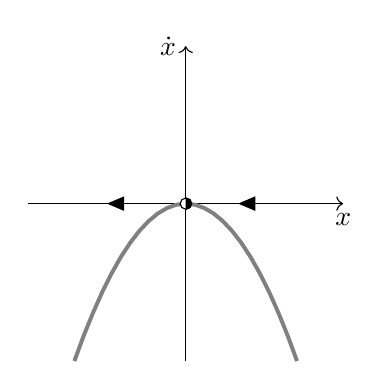
\begin{tikzpicture}[domain=-2:2]
      \draw[->] (-2, 0) -- (2, 0) node[below] {$x$};
      \draw[->] (0, -2) -- (0, 2) node[left] {$\dot{x}$};

      \draw[gray, line width=0.5mm, domain=-1.414:1.414] plot (\x, {- \x*\x});

      \node[circle, fill=white, draw=black, inner sep=0pt, minimum size=4pt] (a) at (0, 0) {};
      \node[semicircle, fill=black, draw=black, inner sep=0pt, minimum size=2pt, rotate=-90, anchor=south] (a) at (0, 0) {};

      \node[rotate=90, inner sep=0pt] () at (-1, 0) {\tikz\draw[-triangle 45](0, 0) ;};
      \node[rotate=90, inner sep=0pt] () at (0.666, 0) {\tikz\draw[-triangle 45](0, 0) ;};

    \end{tikzpicture}

    $$\mu = 0$$
  \end{minipage}%
  \hfill
  \begin{minipage}{.32\textwidth}
    \centering
    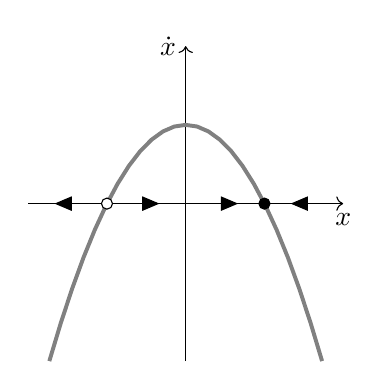
\begin{tikzpicture}[domain=-2:2]
      \draw[->] (-2, 0) -- (2, 0) node[below] {$x$};
      \draw[->] (0, -2) -- (0, 2) node[left] {$\dot{x}$};

      \draw[gray, line width=0.5mm, domain=-1.732:1.732] plot (\x, {1 - \x*\x});

      \node[circle,fill=white, draw=black, inner sep=0pt,minimum size=4pt] (a) at (-1, 0) {};
      \node[rotate=90, inner sep=0pt] () at (-1.666, 0) {\tikz\draw[-triangle 45](0, 0) ;};
      \node[rotate=-90, inner sep=0pt] () at (-0.333, 0) {\tikz\draw[-triangle 45](0, 0) ;};

      \node[circle, fill=black, draw=black, inner sep=0pt,minimum size=4pt] (a) at (1, 0) {};
      \node[rotate=90, inner sep=0pt] () at (1.333, 0) {\tikz\draw[-triangle 45](0, 0) ;};
      \node[rotate=-90, inner sep=0pt] () at (0.666, 0) {\tikz\draw[-triangle 45](0, 0) ;};

    \end{tikzpicture}

    $$\mu = 1$$

  \end{minipage}

  \vspace{1cm}
\end{frame}

\begin{frame}[t, c]{Saddle-node bifurcation}{Motivating example : Over-damped pendulum driven by a constant torque}
  \begin{minipage}{.68\textwidth}
    \begin{itemize}
    \item Starting from Newton's principles, the equation of motion is given by
      %
      \[
      mL^2 \ddot{\theta} + b \dot{\theta} + mgL \sin(\theta) = \Gamma.
      \]
      
    \item Dividing by $mgL$ and rescaling time as $t \to \tau t$ yields
      %
      \[
      \dfrac{L}{g \tau^2} \ddot{\theta} + \dfrac{b}{mgL \tau} \dot{\theta} + \sin(\theta) = \dfrac{\Gamma}{mgL}.
      \]
      
    \item We are now left with two possible choices for the time scale $\tau$.
      
    \end{itemize}
  \end{minipage}%
  \hfill
  \begin{minipage}{.28\textwidth}
    \centering
    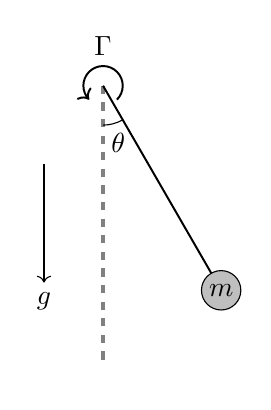
\begin{tikzpicture}
      \coordinate (center) at (0,0);
      \draw[dashed, gray, line width=0.5mm] (center) -- ++ (0,-3.5) node (mary) [black,below]{};

      \draw[line width=0.25mm] (center) -- ++(300:3) coordinate (bob);

      \fill[fill=lightgray, draw=black] (bob) circle (0.25) node[] {$m$};

      \pic [draw, -, "$\theta$", angle eccentricity=1.5] {angle = mary--center--bob};

      \draw[domain=-45:270-45, line width=0.25mm, ->] plot ({0.25*cos(\x)}, {0.25*sin(\x)});
      \node[] at (0, 0.5) {$\Gamma$};

      \draw[->] (-0.75, -1) -- (-0.75, -2.5) node[below] {$g$}; 
    \end{tikzpicture}
  \end{minipage}

\end{frame}

\begin{frame}[t, c]{Saddle-node bifurcation}{Motivating example : Over-damped pendulum driven by a constant torque}
  \begin{minipage}{.68\textwidth}
    If friction is by far the dominant force (over-damped situation), we can approximately reduce our equation to
    %
    \[
    \dot{\theta} = \gamma - \sin(\theta)
    \]
    %
    where $\gamma = \nicefrac{\Gamma}{mgL}$ is our control parameter.
  \end{minipage}%
  \hfill
  \begin{minipage}{.28\textwidth}
    \centering
    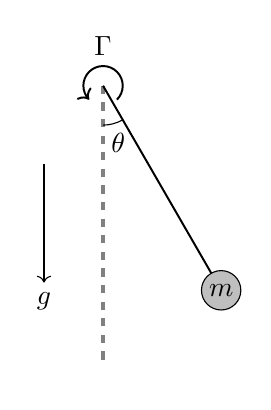
\begin{tikzpicture}
      \coordinate (center) at (0,0);
      \draw[dashed, gray, line width=0.5mm] (center) -- ++ (0,-3.5) node (mary) [black,below]{};

      \draw[line width=0.25mm] (center) -- ++(300:3) coordinate (bob);

      \fill[fill=lightgray, draw=black] (bob) circle (0.25) node[] {$m$};

      \pic [draw, -, "$\theta$", angle eccentricity=1.5] {angle = mary--center--bob};

      \draw[domain=-45:270-45, line width=0.25mm, ->] plot ({0.25*cos(\x)}, {0.25*sin(\x)});
      \node[] at (0, 0.5) {$\Gamma$};

      \draw[->] (-0.75, -1) -- (-0.75, -2.5) node[below] {$g$}; 
    \end{tikzpicture}
  \end{minipage}

  \vspace{1cm}
\end{frame}

\begin{frame}[t, c]{Saddle-node bifurcation}{Motivating example : Over-damped pendulum driven by a constant torque}
  \begin{minipage}{.48\textwidth}

    \begin{overprint}
      \onslide<1>
      \begin{itemize}
      \item When $\gamma$ is sufficiently large, the system has no fixed point.
        
        \bigskip
        
      \item Physically, the applied torque is large enough to cause the pendulum to spin indefinitely.
      \end{itemize}

      \onslide<2>
      \begin{itemize}
      \item For $\gamma = 1$, the torque can barely counter-balance friction and gravity.

        \medskip

      \item A meta-stable fixed point is created.

      \end{itemize}

      \onslide<3>
      In the vicinity of this point, the system can be approximated by
      %
      \[
      \dot{\eta} = \mu + \eta^2
      \]
      %
      with $\mu = \gamma - 1$, hence the name \textbf{normal form}.
        
      \onslide<4>
      \begin{itemize}
      \item For $\vert \gamma \vert < 1$, torque is no longer able to overcome gravity and friction.

        \bigskip

      \item Two equilibrium positions co-exist, a stable and an unstable one.
      \end{itemize}

    \end{overprint}
  \end{minipage}%
  \hfill
  \begin{minipage}{.48\textwidth}
    \begin{overprint}
      \onslide<1>
      \centering
      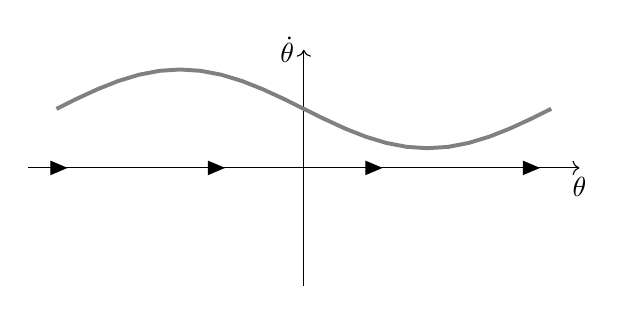
\begin{tikzpicture}
        \draw[->] (-3.5, 0) -- (3.5, 0) node[below] {$\theta$};
        \draw[->] (0, -1.5) -- (0, 1.5) node[left] {$\dot{\theta}$};
        
        \draw[gray, line width=0.5mm, domain=-pi:pi] plot (\x, {0.75 - 0.5*sin(\x r)});
        
        \node[rotate=-90, inner sep=0pt] () at (-3, 0) {\tikz\draw[-triangle 45](0, 0) ;};
        \node[rotate=-90, inner sep=0pt] () at (-1, 0) {\tikz\draw[-triangle 45](0, 0) ;};
        \node[rotate=-90, inner sep=0pt] () at (1, 0) {\tikz\draw[-triangle 45](0, 0) ;};
        \node[rotate=-90, inner sep=0pt] () at (3, 0) {\tikz\draw[-triangle 45](0, 0) ;};
        
      \end{tikzpicture}

      $$\gamma = 1.5$$

      \onslide<2>
      \centering
      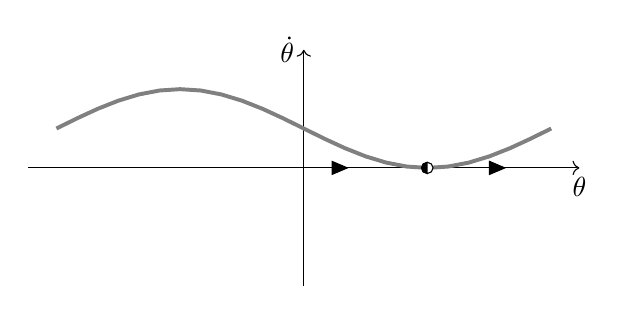
\begin{tikzpicture}
        \draw[->] (-3.5, 0) -- (3.5, 0) node[below] {$\theta$};
        \draw[->] (0, -1.5) -- (0, 1.5) node[left] {$\dot{\theta}$};
        
        \draw[gray, line width=0.5mm, domain=-pi:pi] plot (\x, {0.5 - 0.5*sin(\x r)});

        \node[rotate=-90, inner sep=0pt] () at (pi/2-1, 0) {\tikz\draw[-triangle 45](0, 0) ;};
        \node[rotate=-90, inner sep=0pt] () at (pi/2+1, 0) {\tikz\draw[-triangle 45](0, 0) ;};

        \node[circle, fill=white, draw=black, inner sep=0pt, minimum size=4pt] (a) at (pi/2, 0) {};
        \node[semicircle, fill=black, draw=black, inner sep=0pt, minimum size=2pt, rotate=90, anchor=south] (a) at (pi/2, 0) {};

      \end{tikzpicture}
      
      $$\gamma = 1$$

      \onslide<3>
      \centering
      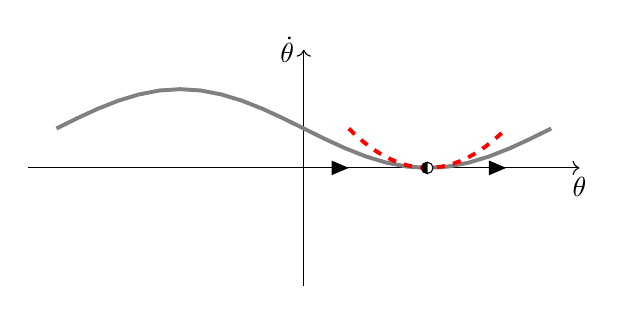
\begin{tikzpicture}
        \draw[->] (-3.5, 0) -- (3.5, 0) node[below] {$\theta$};
        \draw[->] (0, -1.5) -- (0, 1.5) node[left] {$\dot{\theta}$};
        
        \draw[gray, line width=0.5mm, domain=-pi:pi] plot (\x, {0.5 - 0.5*sin(\x r)});

        \draw[red, dashed, line width=0.5mm, domain=pi/2-1:pi/2+1] plot (\x, {0.5*(\x - pi/2)^2});

        \node[rotate=-90, inner sep=0pt] () at (pi/2-1, 0) {\tikz\draw[-triangle 45](0, 0) ;};
        \node[rotate=-90, inner sep=0pt] () at (pi/2+1, 0) {\tikz\draw[-triangle 45](0, 0) ;};

        \node[circle, fill=white, draw=black, inner sep=0pt, minimum size=4pt] (a) at (pi/2, 0) {};
        \node[semicircle, fill=black, draw=black, inner sep=0pt, minimum size=2pt, rotate=90, anchor=south] (a) at (pi/2, 0) {};

      \end{tikzpicture}
      
      $$\gamma = 1$$

      \onslide<4>
      \centering
      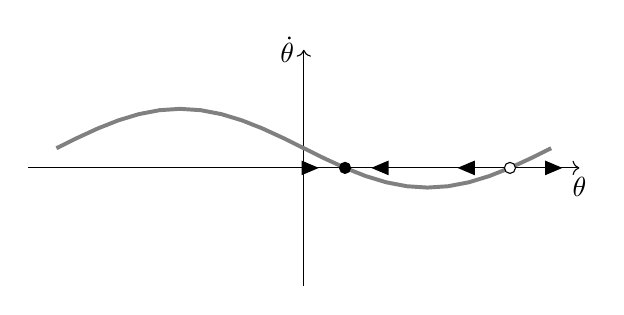
\begin{tikzpicture}
        \draw[->] (-3.5, 0) -- (3.5, 0) node[below] {$\theta$};
        \draw[->] (0, -1.5) -- (0, 1.5) node[left] {$\dot{\theta}$};
        
        \draw[gray, line width=0.5mm, domain=-pi:pi] plot (\x, {0.25 - 0.5*sin(\x r)});
        
        \node[rotate=90, inner sep=0pt] () at (pi/6+0.333, 0) {\tikz\draw[-triangle 45](0, 0) ;};
        \node[rotate=-90, inner sep=0pt] () at (pi/6-0.333, 0) {\tikz\draw[-triangle 45](0, 0) ;};
        \node[circle, fill=black, draw=black, inner sep=0pt, minimum size=4pt] (a) at (pi/6, 0) {};

        \node[rotate=-90, inner sep=0pt] () at (5*pi/6+0.666, 0) {\tikz\draw[-triangle 45](0, 0) ;};
        \node[rotate=90, inner sep=0pt] () at (5*pi/6-0.666, 0) {\tikz\draw[-triangle 45](0, 0) ;};
        \node[circle, fill=white, draw=black, inner sep=0pt, minimum size=4pt] (a) at (5*pi/6, 0) {};

      \end{tikzpicture}
      
      $$\gamma = 0.5$$
      
    \end{overprint}
  \end{minipage}

  \vspace{0.5cm}
\end{frame}

\begin{frame}[t, c]{Pitchfork bifurcation}{Breaking the symmetry}
  \begin{minipage}{.48\textwidth}
    \begin{block}{\centering \alert{\textbf{Supercritical pitchfork bifurcation}}}
      \centering

      \medskip

      \( \dot{x} = \mu x - x^3 \)
    \end{block}

    \bigskip

    \begin{itemize}
    \item For $\mu < 0$, a single stable fixed point exist.

      \medskip

    \item As $\mu$ becomes positive, two stable fixed points are created while the original one becomes unstable.
    \end{itemize}
  \end{minipage}%
  \hfill
  \begin{minipage}{.48\textwidth}
    \centering
    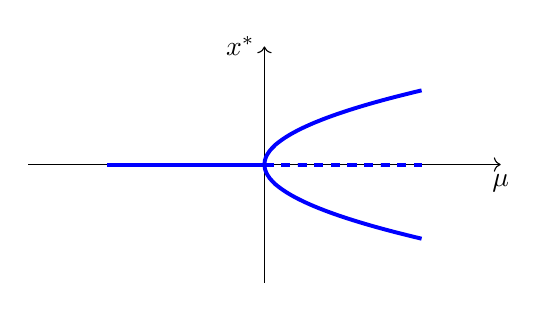
\begin{tikzpicture}
      \draw[->] (-3, 0) -- (3, 0) node[below] {$\mu$};
      \draw[->] (0, -1.5) -- (0, 1.5) node[left] {$x^*$};

      \draw[blue, line width=0.5mm, domain=-2:0, samples=401] plot (\x, {0});
      \draw[blue, dashed, line width=0.5mm, domain=0:2, samples=401] plot (\x, {0});

      \draw[blue, line width=0.5mm, domain=0:2, samples=401] plot (\x, {0.6666*\x^(1/2)});
      \draw[blue, line width=0.5mm, domain=0:2, samples=401] plot (\x, -{0.6666*\x^(1/2)});

    \end{tikzpicture}
  \end{minipage}

  \vspace{1cm}
\end{frame}

\begin{frame}[t, c]{Pitchfork bifurcation}{Breaking the symmetry}
  \begin{minipage}{.32\textwidth}
    \centering
    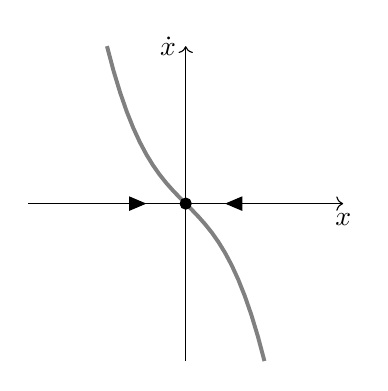
\begin{tikzpicture}[domain=-2:2]
      \draw[->] (-2, 0) -- (2, 0) node[below] {$x$};
      \draw[->] (0, -2) -- (0, 2) node[left] {$\dot{x}$};
      
      \draw[gray, line width=0.5mm, domain=-1:1] plot (\x, {-\x - \x^3});
      
      \node[rotate=-90, inner sep=0pt] () at (-0.5, 0) {\tikz\draw[-triangle 45](0, 0) ;};
      \node[rotate=90, inner sep=0pt] () at (0.5, 0) {\tikz\draw[-triangle 45](0, 0) ;};
      \node[circle, fill=black, draw=black, inner sep=0pt, minimum size=4pt] (a) at (0, 0) {};
      
    \end{tikzpicture}

    $$\mu = -1$$
    
  \end{minipage}%
  \hfill
  \begin{minipage}{.32\textwidth}
    \centering
    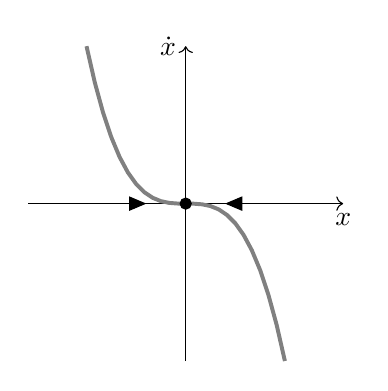
\begin{tikzpicture}[domain=-2:2]
      \draw[->] (-2, 0) -- (2, 0) node[below] {$x$};
      \draw[->] (0, -2) -- (0, 2) node[left] {$\dot{x}$};
      
      \draw[gray, line width=0.5mm, domain=-2^(1/3):2^(1/3)] plot (\x, {- \x^3});
      
      \node[rotate=-90, inner sep=0pt] () at (-0.5, 0) {\tikz\draw[-triangle 45](0, 0) ;};
      \node[rotate=90, inner sep=0pt] () at (0.5, 0) {\tikz\draw[-triangle 45](0, 0) ;};
      \node[circle, fill=black, draw=black, inner sep=0pt, minimum size=4pt] (a) at (0, 0) {};      
    \end{tikzpicture}
    
    $$\mu = 0$$
  \end{minipage}%
  \hfill
  \begin{minipage}{.32\textwidth}
    \centering
    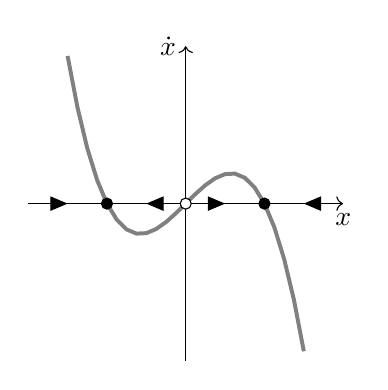
\begin{tikzpicture}[domain=-2:2]
      \draw[->] (-2, 0) -- (2, 0) node[below] {$x$};
      \draw[->] (0, -2) -- (0, 2) node[left] {$\dot{x}$};
      
      \draw[gray, line width=0.5mm, domain=-1.5:1.5] plot (\x, {\x - \x^3});
      
      \node[rotate=90, inner sep=0pt] () at (-0.5, 0) {\tikz\draw[-triangle 45](0, 0) ;};
      \node[rotate=-90, inner sep=0pt] () at (0.5, 0) {\tikz\draw[-triangle 45](0, 0) ;};
      \node[circle, fill=white, draw=black, inner sep=0pt, minimum size=4pt] (a) at (0, 0) {};

      \node[rotate=-90, inner sep=0pt] () at (-1.5, 0) {\tikz\draw[-triangle 45](0, 0) ;};
      \node[circle, fill=black, draw=black, inner sep=0pt, minimum size=4pt] (a) at (-1, 0) {};

      \node[rotate=90, inner sep=0pt] () at (1.5, 0) {\tikz\draw[-triangle 45](0, 0) ;};
      \node[circle, fill=black, draw=black, inner sep=0pt, minimum size=4pt] (a) at (1, 0) {};

    \end{tikzpicture}
    
    $$\mu = 1$$
    
  \end{minipage}
  
  \vspace{1cm}
  
\end{frame}


\begin{frame}[t, c]{Pitchfork bifurcation}{Breaking the symmetry}
  \begin{minipage}{.48\textwidth}
    \begin{block}{\centering \alert{\textbf{Subcritical pitchfork bifurcation}}}
      \centering

      \medskip

      \( \dot{x} = \mu x + x^3 \)
    \end{block}

    \bigskip

    \begin{itemize}
    \item For $\mu < 0$, three fixed points exist, two unstable and one stable.

      \medskip

    \item As $\mu$ becomes positive, two unstable fixed points disappear while the central one becomes unstable.
    \end{itemize}
  \end{minipage}%
  \hfill
  \begin{minipage}{.48\textwidth}
    \centering
    \begin{tikzpicture}
      \draw[->] (-3, 0) -- (3, 0) node[below] {$\mu$};
      \draw[->] (0, -1.5) -- (0, 1.5) node[left] {$x^*$};

      \draw[blue, line width=0.5mm, domain=-2:0, samples=401] plot (\x, {0});
      \draw[blue, dashed, line width=0.5mm, domain=0:2, samples=401] plot (\x, {0});

      \draw[blue, dashed, line width=0.5mm, domain=-2:0, samples=401] plot (\x, {0.6666*\x^(1/2)});
      \draw[blue, dashed, line width=0.5mm, domain=-2:0, samples=401] plot (\x, -{0.6666*\x^(1/2)});

    \end{tikzpicture}
  \end{minipage}

  \vspace{1cm}
\end{frame}

\begin{frame}[t, c]{Pitchfork bifurcation}{Breaking the symmetry}
  \begin{minipage}{.32\textwidth}
    \centering
    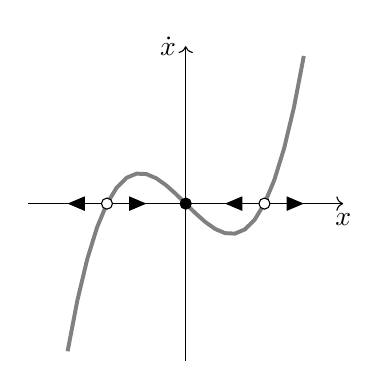
\begin{tikzpicture}[domain=-2:2]
      \draw[->] (-2, 0) -- (2, 0) node[below] {$x$};
      \draw[->] (0, -2) -- (0, 2) node[left] {$\dot{x}$};
      
      \draw[gray, line width=0.5mm, domain=-1.5:1.5] plot (\x, {-\x + \x^3});
      
      \node[rotate=-90, inner sep=0pt] () at (-0.5, 0) {\tikz\draw[-triangle 45](0, 0) ;};
      \node[rotate=90, inner sep=0pt] () at (0.5, 0) {\tikz\draw[-triangle 45](0, 0) ;};
      \node[circle, fill=black, draw=black, inner sep=0pt, minimum size=4pt] (a) at (0, 0) {};

      \node[rotate=90, inner sep=0pt] () at (-1.5, 0) {\tikz\draw[-triangle 45](0, 0) ;};
      \node[circle, fill=white, draw=black, inner sep=0pt, minimum size=4pt] (a) at (-1, 0) {};

      \node[rotate=-90, inner sep=0pt] () at (1.5, 0) {\tikz\draw[-triangle 45](0, 0) ;};
      \node[circle, fill=white, draw=black, inner sep=0pt, minimum size=4pt] (a) at (1, 0) {};

    \end{tikzpicture}

    $$\mu = -1$$
    
  \end{minipage}%
  \hfill
  \begin{minipage}{.32\textwidth}
    \centering
    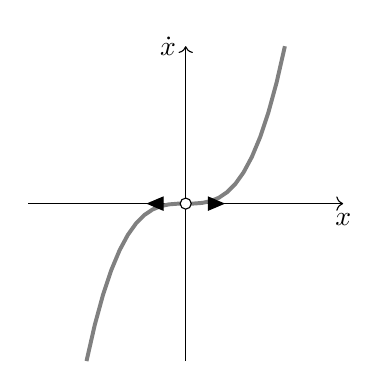
\begin{tikzpicture}[domain=-2:2]
      \draw[->] (-2, 0) -- (2, 0) node[below] {$x$};
      \draw[->] (0, -2) -- (0, 2) node[left] {$\dot{x}$};
      
      \draw[gray, line width=0.5mm, domain=-2^(1/3):2^(1/3)] plot (\x, {\x^3});
      
      \node[rotate=90, inner sep=0pt] () at (-0.5, 0) {\tikz\draw[-triangle 45](0, 0) ;};
      \node[rotate=-90, inner sep=0pt] () at (0.5, 0) {\tikz\draw[-triangle 45](0, 0) ;};
      \node[circle, fill=white, draw=black, inner sep=0pt, minimum size=4pt] (a) at (0, 0) {};      
    \end{tikzpicture}
    
    $$\mu = 0$$
  \end{minipage}%
  \hfill
  \begin{minipage}{.32\textwidth}
    \centering
    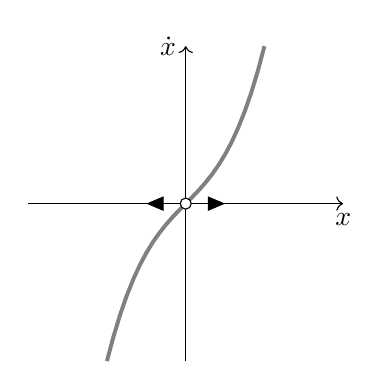
\begin{tikzpicture}[domain=-2:2]
      \draw[->] (-2, 0) -- (2, 0) node[below] {$x$};
      \draw[->] (0, -2) -- (0, 2) node[left] {$\dot{x}$};
      
      \draw[gray, line width=0.5mm, domain=-1:1] plot (\x, {\x + \x^3});
      
      \node[rotate=90, inner sep=0pt] () at (-0.5, 0) {\tikz\draw[-triangle 45](0, 0) ;};
      \node[rotate=-90, inner sep=0pt] () at (0.5, 0) {\tikz\draw[-triangle 45](0, 0) ;};
      \node[circle, fill=white, draw=black, inner sep=0pt, minimum size=4pt] (a) at (0, 0) {};

    \end{tikzpicture}
    
    $$\mu = 1$$
    
  \end{minipage}
  
  \vspace{1cm}
  
\end{frame}

\begin{frame}[t, c]{Subcritical pitchfork bifurcation}{Break the symmetry and the hysteresis phenomenon}
  \begin{minipage}{.58\textwidth}
    \begin{itemize}
    \item For $\mu > 0$, $x(t) \to \pm \infty$ in finite-time.
      It is the \textbf{finite blow-up} phenomenon we mentionned in L2.

      \medskip

    \item In most real systems, this is unphysical and our simple model needs to be modified.

      \medskip

    \item Assuming the system is still symmetric under $x \to -x$, the simplest modification is
      %
      \[
      \dot{x} = \mu x + x^3 - x^5.
      \]
      %
      The analysis of this sytem and of the resulting hysteresis phenomenon is left as an exercise.
    \end{itemize}
  \end{minipage}%
  \hfill
  \begin{minipage}{.38\textwidth}
    \centering
    \begin{tikzpicture}
      \draw[->] (-3, 0) -- (3, 0) node[below] {$\mu$};
      \draw[->] (0, -1.5) -- (0, 1.5) node[left] {$x^*$};

      \draw[blue, line width=0.5mm, domain=-2:0, samples=401] plot (\x, {0});
      \draw[blue, dashed, line width=0.5mm, domain=0:2, samples=401] plot (\x, {0});

      \draw[blue, dashed, line width=0.5mm, domain=-2:0, samples=401] plot (\x, {0.6666*\x^(1/2)});
      \draw[blue, dashed, line width=0.5mm, domain=-2:0, samples=401] plot (\x, -{0.6666*\x^(1/2)});

    \end{tikzpicture}
  \end{minipage}

  \vspace{1cm}
\end{frame}

\begin{frame}[t, c]{One system -- multiple bifurcations}{Example by J. Nathan Kutz}
  \begin{minipage}{.38\textwidth}
    \begin{center}
      \textbf{Example :} \( \dfrac{dx}{dt} = -x \left( x^2 - 2x - \mu \right) \)
    \end{center}
 
    \bigskip

    A \textbf{saddle-node bifurcation} occurs at $\mu = -1$ while a transcritical one occurs at $\mu = 0$.

    \bigskip

    For $\mu \geq -1$, the system can exhibit \textbf{hysteresis} and \textbf{bi-stability}.

  \end{minipage}%
  \hfill
  \begin{minipage}{.58\textwidth}
    \centering
    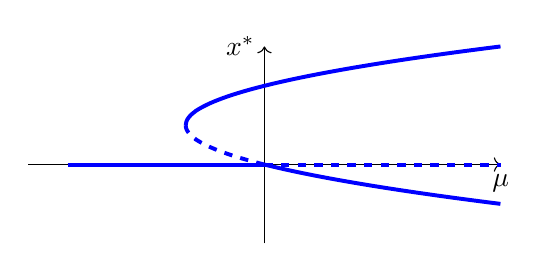
\begin{tikzpicture}
      \draw[->] (-3, 0) -- (3, 0) node[below] {$\mu$};
      \draw[->] (0, -1) -- (0, 1.5) node[left] {$x^*$};
      
      \draw[blue, line width=0.5mm, domain=-1:3, samples=401] plot (\x, {0.5*(1 + (1 + \x)^(1/2))});
      \draw[blue, dashed, line width=0.5mm, domain=-1:0, samples=401] plot (\x, {0.5*(1 - (1 + \x)^(1/2))});
      \draw[blue, line width=0.5mm, domain=0:3, samples=401] plot (\x, {0.5*(1 - (1 + \x)^(1/2))});
      
      \draw[blue, line width=0.5mm] (-2.5, 0) -- (0, 0) {};
      \draw[blue, dashed, line width=0.5mm] (0, 0) -- (3, 0) {};
      
    \end{tikzpicture}
  \end{minipage}

  \vspace{1cm}
\end{frame}

\end{document}
